% DO NOT COMPILE THIS FILE DIRECTLY!
% This is included by the other .tex files.

\begin{frame}[t,plain]
\titlepage
\end{frame}
%
% PRIMA SLIDE
%
\begin{frame}[t]{\textsc{Introduzione al problema PL}}
\textbf{Modello LP standard:} $A \in \mathbb{R}^{m,n}$ a rango pieno, $c\in \mathbb{R}^{n}, b \in \mathbb{R}^{m}$\\
\begin{equation*}
\begin{split}
\min\;&c^{T}x\\
\text{tale\;che\;}&Ax= b\;\text{e\;}x\geq0
\end{split}
\end{equation*}
\pause
\text{L'insieme dei punti ammissibili è:}\\
\begin{equation*}
\mathcal{P}=\lbrace x\in\mathbb{R}^{n}\; |\; Ax = b , x \geq0\rbrace
\end{equation*}
Il valore ottimale è il valore $c^{T}x^{*}=\min\limits_{x\in\mathcal{P}}c^{T}x$
\\ e $x^{*}$ è detta soluzione ottimale.
\end{frame}

%
% SECONDA SLIDE
%
\begin{frame}
\text{Ipotesi: $m \leq n$} \pause $\longrightarrow m\times m $ \text{sottomatrice di A invertibile, }$\mathbf{A_{B}}$ \\ \text{     con }$B\subseteq\{1,\dots,n\}$ \\
\pause
\text{Partizione (B,N):}\\
\begin{center}
$\text{min\;} c^{T}_{B}x_{B}+c^{T}_{N}x_{N}$,\\
\text{tale\;che\;}$A_{B}x_{B}+A_{N}x_{N} = b$\text{\;e\;}$x_{B}, x_{N}\geq0$
\end{center}
\pause
\text{Soluzione di base }$(x_{B},x_{N})=(A_{B}^{-1}b,0_{[N]})$. \text{Se}$\;A_{B}^{-1}b>0$
\text{ allora è detta soluzione non degenere, altrimenti soluzione degenere.}
\end{frame}
%
% TERZA SLIDE
%
\begin{frame}[t]{\textsc{Teorema fondamentale della PL}}
\pause
Ogni problema di PL in forma standard soddisfa solo una delle seguenti:
\begin{itemize}
	\item se ha una soluzione ottima allora è una soluzione ammssibile di base; 
	%che ha valore minore o uguale a qualunque altro punto ammissibile;
	\item è illimitato;
	\item non ha punti ammissibili.
\end{itemize}
\end{frame}
%
% QUARTA SLIDE
%
\begin{frame}{Esempio di problema PL}
\begin{columns}
\begin{column}{.6\textwidth}
$\min\limits_{(x_{1},x_{2},x_{3})\in\mathbb{R}^{3}} -x_{1}+ x_{2}-4x_{3}$\\
\text{tale che    }$x_{1}+x_{2}+x_{3}=1$\\
\text{ con   } $x_{1}, x_{2}, x_{3} \geq 0$
\end{column}
\pause
\begin{column}{.4\textwidth}
\text{Regione ammissibile $\mathcal{P}$}
\text{e le soluzioni di base}
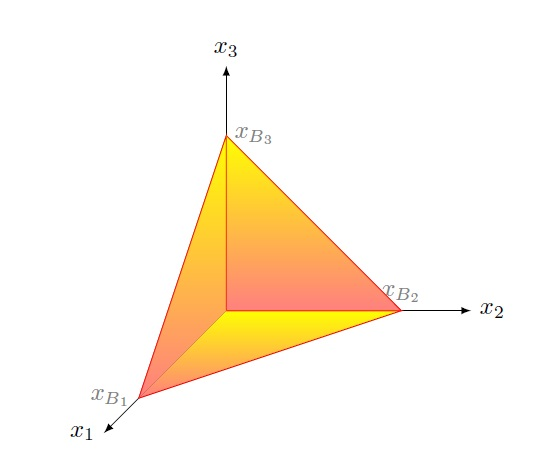
\includegraphics[width=\columnwidth]{Feas.jpg}
\end{column}
\end{columns}
\end{frame}
%
% QUINTA SLIDE
%
\begin{frame}{\textsc{Metodo del Simplesso}}
\begin{itemize}
	\pause
	\item Dantzig 1947
	\pause
	\item si basa sul Teorema Fondamentale:
	esplora solo le soluzioni ammissibili di base; 
	\pause
	\item ad ogni iterazione c'è un cambiamento di base di una sola entrata: \\da un vertice al vertice adiacente $\rightarrow$ pivoting;
	\pause
	\item raggiunge
	il valore ottimale, se esiste, in un numero finito di iterazioni;
	\pause
	\item casi di degenerazione $\rightarrow$ regola di Bland. 
\end{itemize}
\end{frame}
%
% SESTA SLIDE
%
\begin{frame}{\textsc{Metodo del Simplesso}: Test di ottimalità}
Dato un PL e una base ammissibile B: se $c_{N}$ è non
negativa (non positivi) la soluzione di base ammissibile
$x_{B} = B^{-1}b \geq 0$, $x_{N} = 0$ è ottimale.
Infatti, se
$c_{N}^{T} \geq 0$:\\
allora $c^{T}x = c^{T}_{B} B^{-1}b + c^{T}_{N}x_{N} \geq c^{T}_{B}B^{-1}b$.
\end{frame}

\begin{frame}{\textsc{Metodo del Simplesso}: Limiti}

\end{frame}

\begin{frame}[t,fragile]{How to use the theme}
\begin{itemize}
\item Install Beamer
  \begin{itemize}
  \item Some distros have a \verb!latex-beamer! package
  \end{itemize}
\item Read the Beamer documentation
  \begin{itemize}
  \item \verb!/usr/share/doc/latex-beamer/beameruserguide.pdf.gz! if you are
        using Debian
  \item \verb!doc/beameruserguide.pdf! in the source package
  \end{itemize}
\item Install the theme
  \begin{itemize}
  \item \verb!mkdir -p ~/texmf/tex/latex/beamer!\\
  \item \verb!cp *.sty ~/texmf/tex/latex/beamer!
  \end{itemize}
\item Read the example files
  \begin{itemize}
  \item \verb!chameleon.tex!: green theme, watermark and circles for bullet
        lists
  \item \verb!nouvelle.tex!: green and red theme, watermark and squares for
        bullet lists
  \item \verb!freewilly.tex!: blue theme, a logo and squares for bullet lists
  \end{itemize}
\end{itemize}
\end{frame}

\begin{frame}[t,fragile]{Theme files}
\begin{itemize}
\item Themes are composed by sub-themes for single features
\item Inner themes define how the title page, the bullet lists, margins,
      etc. work
  \begin{itemize}
    \item \verb!beamerinnerthemefancy.sty!
  \end{itemize}
\item Outer themes define how headers and footers look like
  \begin{itemize}
    \item \verb!beamerouterthemedecolines.sty!
  \end{itemize}
\item Color themes define the colors to be used in outer and inner themes
  \begin{itemize}
    \item \verb!beamercolorthemechameleon.sty!: green footers and headers
    \item \verb!beamercolorthemenouvelle.sty!: green footers, red headers and
          and frame title
    \item \verb!beamercolorthemefreewilly.sty!: blue footers, headers and
          frame title
  \end{itemize}
\item Global themes just include inner, outer and color themes
  \begin{itemize}
    \item \verb!beamerthemeTorino.sty!
  \end{itemize}
\end{itemize}
\end{frame}

\begin{frame}[t,fragile]{Configuring the theme}
\begin{itemize}
\item Beamer themes can be configured with options between \verb![! and
      \verb!]!
  \begin{itemize}
  \item \verb!\usetheme[option1 = value, option2 = value]{Torino}!
  \end{itemize}
\item If you do not specify any option, you get
  \begin{itemize}
  \item Simple title page
  \item No watermark or logo
  \item Chameleon (green) color theme
  \item Squares for bullet lists
  \end{itemize}
\item Color themes can be changed with \verb!\usecolortheme!
  \begin{itemize}
  \item \verb!\usecolortheme{nouvelle}!: green and red
  \item \verb!\usecolortheme{freewilly}!: blue
  \end{itemize}
\item A logo, shown in the upper right corner, can be choosen with the
      \verb!\logo! command
  \begin{itemize}
  \item \verb!\logo{\includegraphics[height=50px]{logo-image}}!
  \end{itemize}
\end{itemize}
\end{frame}

\begin{frame}[t,fragile]{Alternative title page}
\begin{itemize}
\item A fancy title page can be enabled with the \verb!alternativetitlepage!
      option
\item You can put a logo in the title page, just pass the file name using the
      \verb!titlepagelogo! option
\item Remember to use a plain and top-aligned frame when using alternative title
      pages:\\
      \vskip1ex
      \verb!\begin{frame}[t,plain]!\\
      \verb!\titlepage!\\
      \verb!\end{frame}!
\end{itemize}
\end{frame}

\begin{frame}[t,fragile]{Watermark}
\begin{itemize}
\item A watermark can be shown in the bottom right corner of frames
\item Use the \verb!watermark! option to set name of the image file
\item The \verb!watermarkheight! option specifies the height of the watermark
      image
\item It's a good idea to have a big image and shrink it, so it looks good
      when the slide is full screen
\item If the image height in the slide is not the same as the original one,
      you have to use the \verb!watermarkheightmult! option
  \begin{itemize}
  \item For example, if the image is 400 pixel tall but you want it to
        occupy only 100 pixels, use
        \verb![watermarkheight=100px, watermarkheightmult=4]!
  \item It's ugly but I don't know how to fix it
  \end{itemize}
\end{itemize}
\end{frame}

\watermarkoff
\begin{frame}[t,fragile]{Disabling the watermark}
\begin{itemize}
\item You may want to disable the watermark on some frames
  \begin{itemize}
  \item For example, an image could partially cover the watermark, with ugly
        results
  \end{itemize}
\item The \verb!\watermarkoff! command can be used to disable the watermark
      in the following frames
\item The \verb!\watermarkon! command restores the watermark in the following
      frames
\item If you did not specify a watermark, nothing happens
\vskip5ex
\item \verb!\watermarkoff! was used for this frame
\end{itemize}
\end{frame}
\watermarkon

\begin{frame}[t,fragile]{Other options}
\begin{itemize}
\item The \verb!pageofpages! option defines the string between the current
      page number and the total page count
  \begin{itemize}
  \item The default is ``/''
  \item The example files set \verb!pageofpages! to ``of''
  \end{itemize}
\item The \verb!bullet! option can be used to choose the symbol used in
      bullet lists
  \begin{itemize}
  \item \verb!square!: A filled square
        ({\usebeamercolor[fg]{item}\tiny\raise0.2ex\hbox{$\blacksquare$}}) for
        first and third level items, an empty square
        ({\usebeamercolor[fg]{item}\tiny\raise0.2ex\hbox{$\square$}}) for
        second level items
  \item \verb!circle!: A filled circle ({\usebeamercolor[fg]{item}$\bullet$})
        for first and third level items, an empty circle
        ({\usebeamercolor[fg]{item}$\circ$}) for second level items
  \item The default value is \verb!square!
  \end{itemize}
\item If the \verb!titleline! option is set to \verb!true!, a horizontal line
      is drawn below the title
\end{itemize}
\end{frame}

